\documentclass[tikz,border=3pt]{standalone}
\usepackage[utf8]{inputenc}
\usepackage[T1]{fontenc}
\usepackage{lmodern}
\renewcommand{\familydefault}{\sfdefault}
\usepackage{sansmath}\sansmath
\usepackage{chemfig}
\usepackage{pgfplots}\pgfplotsset{compat=1.18,/pgf/number format/use comma,/pgf/number format/1000 sep={.}}
\usetikzlibrary{arrows.meta,calc,positioning,decorations.pathmorphing,patterns}
% paleta del sitio
\definecolor{nar}{HTML}{E8680C}\definecolor{narc}{HTML}{FFB35C}\definecolor{hielo}{HTML}{FFF3E8}
\definecolor{tinta}{HTML}{1D1D1F}\definecolor{gris}{HTML}{6E6E73}\definecolor{lila}{HTML}{7C5CF0}
\definecolor{azul}{HTML}{2F6FD6}\definecolor{menta}{HTML}{17A673}\definecolor{coral}{HTML}{E8342A}
\begin{document}
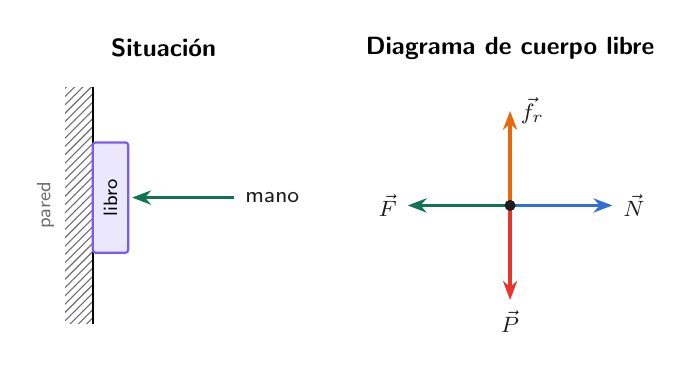
\begin{tikzpicture}[font=\footnotesize,>={Stealth[length=2.4mm]}]
% situación
\node[font=\small\bfseries] at (0.9,2.6) {Situación};
\fill[pattern=north east lines,pattern color=gris] (-0.35,-0.9) rectangle (0,2.1);
\draw[thick] (0,-0.9) -- (0,2.1);
\node[gris,font=\scriptsize,rotate=90] at (-0.6,0.6) {pared};
\draw[thick,draw=lila,fill=lila!15,rounded corners=1pt] (0,0) rectangle (0.45,1.4);
\node[rotate=90,font=\scriptsize] at (0.225,0.7) {libro};
\draw[->,very thick,menta!70!black] (1.8,0.7) -- (0.5,0.7) node[pos=0,right,text=tinta] {mano};
% diagrama de cuerpo libre
\node[font=\small\bfseries] at (5.3,2.6) {Diagrama de cuerpo libre};
\coordinate (c) at (5.3,0.6);
\draw[->,very thick,menta!70!black] (c) -- ++(-1.3,0) node[left,text=tinta] {$\vec F$};
\draw[->,very thick,azul] (c) -- ++(1.3,0) node[right,text=tinta] {$\vec N$};
\draw[->,very thick,coral] (c) -- ++(0,-1.2) node[below,text=tinta] {$\vec P$};
\draw[->,very thick,nar] (c) -- ++(0,1.2) node[right,text=tinta] {$\vec f_r$};
\fill[tinta] (c) circle (2pt);
\end{tikzpicture}
\end{document}
